\section{Graphentheorie}

Ein grundlegendes, strukturelles Verständniss von Graphen ist wichtig für diese Arbeit, da diese mathematische Struktur
die Grundlage der gesamten Arbeit bildet. In diesem Kapitel werden viele Definitionen mithilfe eines mathematischen
Lehrbuchs erarbeitet. Es wird später ersichtlich werden wozu diese Definitionen wichtig sind auch wenn diese jetzt noch
sehr abstrakt erscheinen.

\subsection{allgemeiner Graph}

Ein Graph ist ein Paar \textrm{G = (V, E)} zweier disjunkter Mengen (vgl. Graphlehrbuch) mit E \subseteq V^2 (vgl. Graphlehrbuch)

Elemente von V nennt man Knoten eines Graphens, die Elemente von E nennt man Kanten, Knoten die in einem Tupel von E vorkommen
nennt man auch inzident (benachbart).
Ein Graph könnte man nun definieren indem wir z.B. für V = {1, 2, 3} wählen und für E = {(1, 1), (1, 2), (1, 3)}.
Dargestellt werden können Graphen indem man die Elemente von V als z.B. Kreis zeichnet und dann alle Kanten aus E
einzeichnet indem man die Punkte verbindet. Eben definierter Graph hat z.B. folgende Darstellung:

\begin{center}
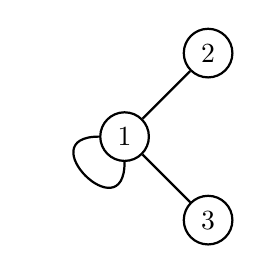
\begin{tikzpicture}[node distance={15mm}, thick, main/.style = {draw, circle}]
    \node[main] (1) {$1$};
    \node[main] (2) [above right of=1] {$2$};
    \node[main] (3) [below right of=1] {$3$};
    \draw (1) to [out=180,in=270,looseness=5] (1);
    \draw (1) -- (2);
    \draw (1) -- (3);
\end{tikzpicture}
\end{center}

Mit dieser Definition lassen sich nun beliebig große Graphen erstellen.
Einige Eigenschaften von Graphen müssen nun noch genau definiert werden da diese später relevant sein werden.
Zu definieren sind Wege und Kreise, gerichtetheit von Kanten und Zusammenhang von Graphen

\subsection{Gerichtetheit von Kanten}

Die vorher getroffene Definition eines Graphens ist im Allgemeinen die Definition eines ungerichteten Graphens.
In einem ungerichteten Graphen bedeutet die Notation E = {(1,2)} das ein Weg von Knoten 1 zu 2 und von 2 zu 1 existiert.
Es muss in diesem Fall nur eine Kante angegeben werden und trotzdem existieren Wege für beide Knoten.
Im Kontext eines gerichteten Graphens existiert dann bei einer Kante E = {(1,2)} nur ein Weg von Knoten 1 zu 2.
Graphisch wird dies in einem Graphen deutlich indem man diesen mit Pfeilen zeichnet. Hierbei zeigt der Pfeil auf das Ziel
der Kante. (vgl. Graphlehrbuch)






\subsection{Wege und Kreise}

\subsection{Erreichbarkeit}

\subsection{Zusammenhang von Graphen}

